\documentclass[sigplan,screen]{acmart}

\usepackage[utf8]{inputenc}
\usepackage{microtype}

\AtBeginDocument{%
  \providecommand\BibTeX{{%
    \normalfont B\kern-0.5em{\scshape i\kern-0.25em b}\kern-0.8em\TeX}}}

%%% The following is specific to SPLASH-E '20 and the paper
%%% 'CSS Instruction Enhanced by Objective Typography'
%%% by Karl Stolley.
%%%
\setcopyright{acmlicensed}
\acmPrice{15.00}
\acmDOI{10.1145/3426431.3428656}
\acmYear{2020}
\copyrightyear{2020}
\acmSubmissionID{splashe20main-id5-p}
\acmISBN{978-1-4503-8180-2/20/11}
\acmConference[SPLASH-E '20]{Proceedings of the 2020 ACM SIGPLAN SPLASH-E Symposium}{November 20, 2020}{Virtual, USA}
\acmBooktitle{Proceedings of the 2020 ACM SIGPLAN SPLASH-E Symposium (SPLASH-E '20), November 20, 2020, Virtual, USA}



\begin{document}
\title[CSS Instruction Enhanced by Objective Typography]{CSS Instruction Enhanced by Objective Typography}

\author{Karl Stolley}
\email{kstolley@iit.edu}
\orcid{1234-5678-9012}
\affiliation{
  \institution{Illinois Institute of Technology}
  \streetaddress{Institution Street Address}
  \city{Chicago}
  \state{IL}
  \country{USA}
  \postcode{60616}}

\begin{abstract}
This course experience report details the teaching of Cascading Style Sheets (CSS) constrained by the rules of objective typography. The approach guides students in applying those rules to a subset of fewer than a dozen CSS properties. Students learn how to determine and reason about rule-governed values and ratios according to typographic principles. When successful, students produce typeset text that is accessible and readable across the range of screens and user-set preferences on web-enabled devices. Students learn to visually and mathematically verify the execution of their designs, and to apply the rules of objective typography to other areas of CSS, such as grid-based page layout. Experiential evidence suggests that these techniques do transfer to other aspects of CSS, but formal study is needed.
\end{abstract}

\begin{CCSXML}
<ccs2012>
<concept>
  <concept_id>10003456.10003457.10003527.10003531.10003535</concept_id>
  <concept_desc>Social and professional topics~Information technology education</concept_desc>
  <concept_significance>500</concept_significance>
</concept>
<concept>
  <concept_id>10003456.10003457.10003527.10003528</concept_id>
  <concept_desc>Social and professional topics~Computational thinking</concept_desc>
  <concept_significance>300</concept_significance>
</concept>
</ccs2012>
\end{CCSXML}

\ccsdesc[500]{Social and professional topics~Information technology education}
\ccsdesc[300]{Social and professional topics~Computational thinking}

\keywords{Cascading Style Sheets, typography, web design, curriculum}


\maketitle

\section{Introduction}

At least two factors make CSS a challenging language to teach. First, CSS bears little resemblance to other languages in the web curriculum. HTML traces its ancestry to SGML and its contemporaries to XML. JavaScript has a complicated history but shares features with many prototyped, procedural languages. By contrast, CSS’s closest relative is an obscure one: Simple Tree Transformation Sheets \cite{w3c:briefhistory}, which inspired CSS's selector-declaration syntax.

Second, CSS is a challenge to teach because the language continues to grow. Since the original CSS specification was published in late 1996, the CSS language has expanded considerably in capability as well as complexity: the 53 properties in the CSS 1 specification more than doubled to 115 in CSS 2.1/2.2. The modules that comprise CSS3 included  363 properties \cite{jom:css}. As of October 2020, the World Wide Web Consortium (W3C) estimates that CSS contains or is proposed to contain 533 distinct properties, spread across 145 different technical reports and editors' drafts \cite{w3c:iop}.

 Students also face their own challenges learning CSS. As the language has grown, overwhelmed students often skip the fundamentals in favor of searching for tutorials that delve into complicated visual effects and gimmicks, such as parallax scrolling, which inevitably lead to a lot of cut-and-paste code and little transferable learning.

CSS instruction constrained by typographic principles addresses the  complexity of CSS and attempts to solve the following problems students routinely face learning CSS:

\begin{itemize}
  \item \textbf{Where to start?} CSS can specify many visual qualities,  in just about any order. CSS neither enforces an order nor establishes any given properties as necessary, in contrast to the precise requirements of HTML.
  \item \textbf{What values and units to use?} Left to their own devices, students pick values arbitrarily or from other, inappropriate contexts: {\itshape Google Docs defaults to a text size of 11, so I’ll use 11 on this website, too.}
  \item \textbf{When is it “finished”?} Compared to a set of CSS style declarations, the content-completeness of an HTML document or the feature-completeness of a JavaScript function is more obvious, even to beginners.
\end{itemize}

The instructional approach described here developed out of an effort to teach CSS as equally systematic and rule-governed as well written HTML and JavaScript. Students encounter CSS at a critical moment in the course, when they have become more confident in their HTML skills and are eagerly looking to create their own custom page designs. While this approach is only one part of the course, all the course material that follows hinges on it.

\section{Instructional Context}

This approach has been used several times over a four-year period in the first course of a two-course sequence in introductory web-development. Both courses in the sequence teach accessibility as a core web-engineering principle. The first course, Fundamentals of Web Development, covers the syntax and semantics of standards-based HTML, CSS, and JavaScript. The second course, Human-Computer Interaction and Web Design, introduces theories of user-centered design and human-computer interaction, anchored to common web design problems. The sequence is required for all undergraduate majors in an information technology and management program, and students typically take it in their second year.

The Fundamentals of Web Development course typically enrolls between 30 and 40 students. Classroom instruction is largely lecture based, featuring live-coded demonstrations with ample opportunity for student questions. Students complete between five and ten small lab assignments, including one on objective typography and CSS, which are discussed on the course's electronic discussion boards. A copy of the complete course syllabus is available on the web \cite{kas:fwd}.

The majority of student work in the course, however, is organized around three major projects, completed by each student individually. The first project requires students to develop the semantic HTML foundation for a multi-page website. Students are free to choose the subject matter of their sites, which has lead to substantial student investment in the major course projects. Most students opt to begin developing a professional web presence for themselves, while others choose to create websites for campus clubs or their family's business. The second project adds CSS and audio-visual elements to the HTML work completed in the first project, which students continue to refine and improve. The third project is a significant revision of the second project in response to multiple rounds of peer and instructor feedback, and it requires students to include a JavaScript feature.

\subsection{Objective Typography Principles}

Typography is a familiar design feature for students. They may not have worked with color theory or page layout before, but all have selected a preferred typeface in a document or a slide template. Typography also functions at a human scale, making it a useful constant when designing for the web across the range of wearable, handheld, and desktop devices.

Objective rules for the use of type--“the correct spaces between letters and words and the length and spacing of lines conducive to easy reading” \cite[p.~19]{mb:grid}--trace their origins to the at least the Industrial Revolution. The rules receive exacting description in the work of mid-twentieth-century European designers such as Josef Müller-Brockmann’s {\itshape Grid Systems in Graphic Design}, which labeled the rules as constituting “objective typography” \cite[p.~7]{mb:grid}.

The basic rules of objective typography are refined across a number of contemporary book-length works that I have assigned in web development classes: Ellen Lupton’s {\itshape Thinking with Type}, Robert Bringhurst’s {\itshape The Elements of Typographic Style}, and Jason Santa Maria’s {\itshape On Web Typography} \cite{el:type,rb:style,jsm:owt}. An open-access book that has also been a student favorite is Matthew Butterick’s {\itshape Practical Typography} \cite{mb:pt}. Each of these titles has worked equally well. It is essential only that students read a reference that reinforces the rules of objective typography and explains their underlying principles.

\subsection{Instructional Approach in Brief}

Applying the rules of objective typography to CSS focuses students on determining two values--a font size and a line height--and initially applying those values to fewer than a dozen CSS properties. The font size is chosen from a narrow range of readable values: too small, and the text is difficult to perceive, let alone read. Too large, and too few words appear on a single line, which also hampers reading. The line height, which is selected for comfortable reading based in part on the font size, establishes a predictable, repeating baseline--known as the typographic grid--for text to sit upon. 

Of course, text set at a single size on a uniform grid is neither exciting nor pleasant to read, so students learn to apply a ratio to their base font size to arrive at precise values for larger text (headings, for example) and smaller text (captions and fine print). Those alternative type sizes are always anchored by the original readable, accessible base font size. Students also learn to add additional space above and below headings, list items, and other structural features. That additional space is always some fraction or multiple of the line-height value.

\section{Instructional Method and Experiences}

Applied to CSS instruction, objective typography offers a number of advantages:

\begin{itemize}
  \item It is rule- and principle-governed, which clarifies the objectives of both instruction and assessment
  \item It limits the scope of initial CSS instruction to just a handful of properties and techniques
  \item It exposes students to numerous features of the CSS language, especially inheritance, where a value set on one property affects the initial value or behavior of another, even when set on a different CSS selector
  \item It introduces students to the process of translating and transposing external rules or visual plans from abstract concepts to concrete declarations in CSS
  \item It establishes a set of values and units that anchor advanced CSS methods for grid-based page layout
\end{itemize}

Teaching CSS constrained by objective typography is systematic but leaves open room for experimentation: Students work with both their own written copy and dummy {\itshape Lorem ipsum} text to determine a reasonable size for the body copy, initially expressed in absolute, pixel units. Students begin by setting the necessary CSS properties for the entire page, on the \verb|html| selector.

Because even commonly available typefaces vary between operating systems, students should be encouraged to choose from a few instructor-approved web-available typefaces from a provider such as Google Fonts. Ideally, the candidate typefaces should have anatomical features that lend themselves to long-form reading: moderate stroke contrast, a larger x-height, and pronounced ascenders and descenders \cite[p.~36]{jsm:owt}. The typeface in Figure \ref{fig:rdv-narrow}, Fira Sans, exhibits each of those features and can be viewed on Google Fonts \cite{gf:fs}.

 After applying a reset stylesheet \cite{em:rc}, which strips away all built-in browser styles, students are shown how to work with a mobile-sized viewport to set type for small screens first. Besides being sound development practice, mobile-first design is effectively limited to a single column of text. Multi-column layouts come later in the course.

\subsection{Devices and Viewports}

\begin{figure}
  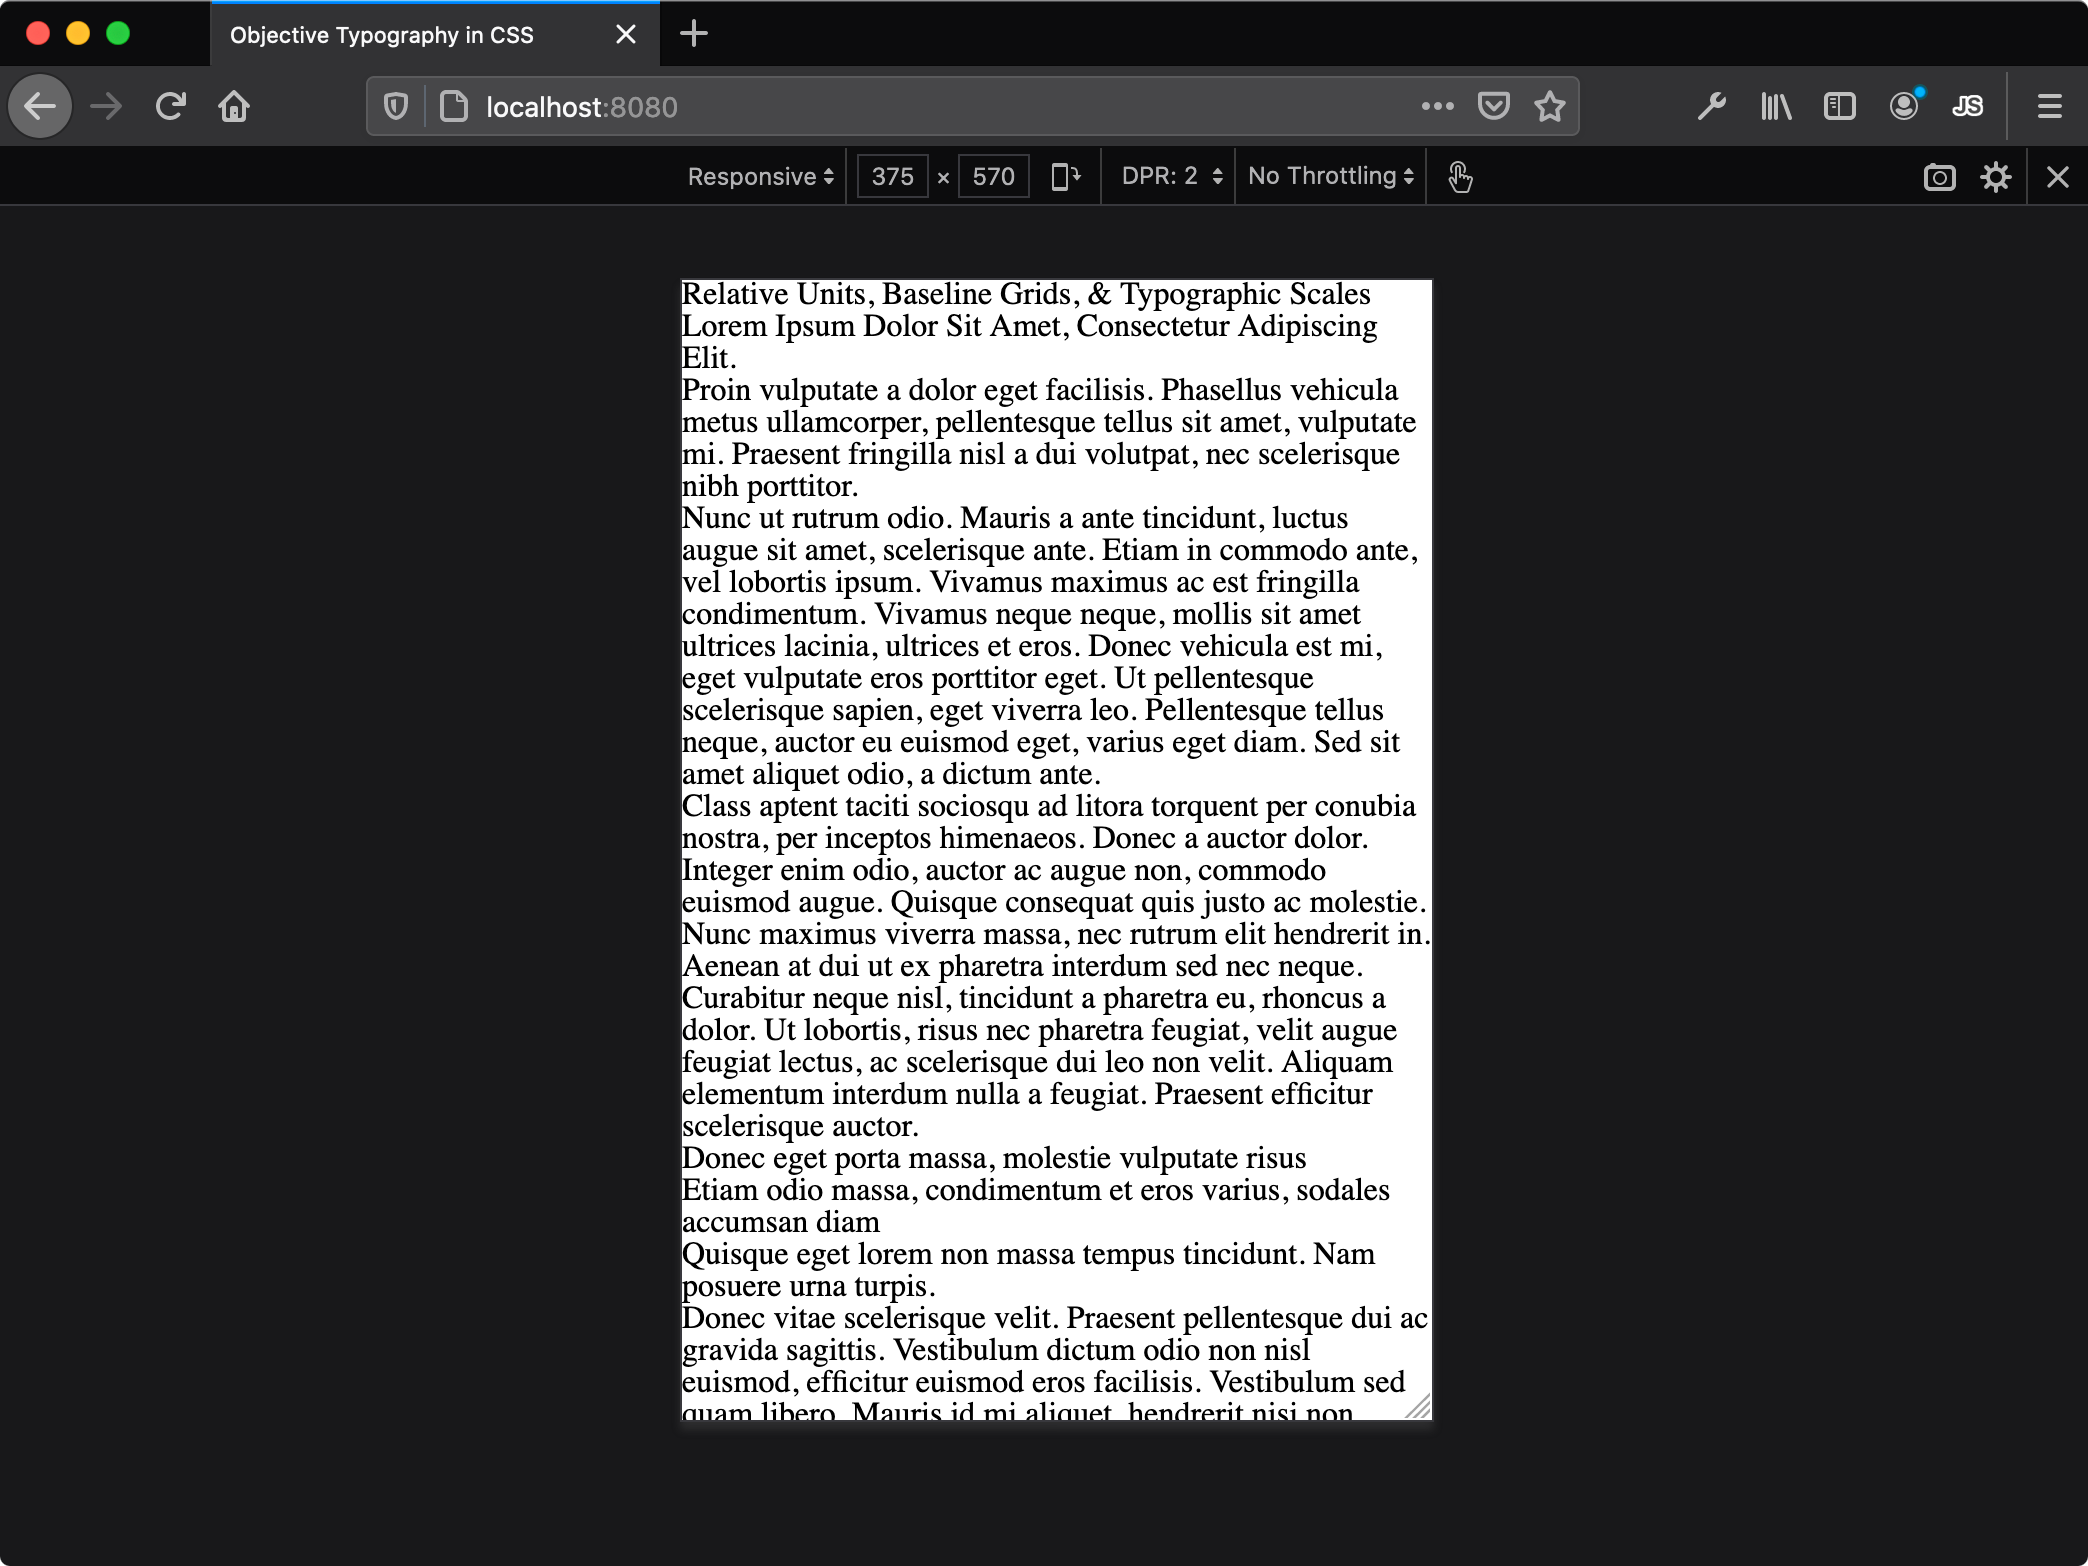
\includegraphics[width=\linewidth]{rdv}
  \caption{The responsive design view (RDV) in Mozilla Firefox. The  page displayed has only a reset stylesheet applied.}
  \label{fig:rdv}
\end{figure}

\begin{figure}
  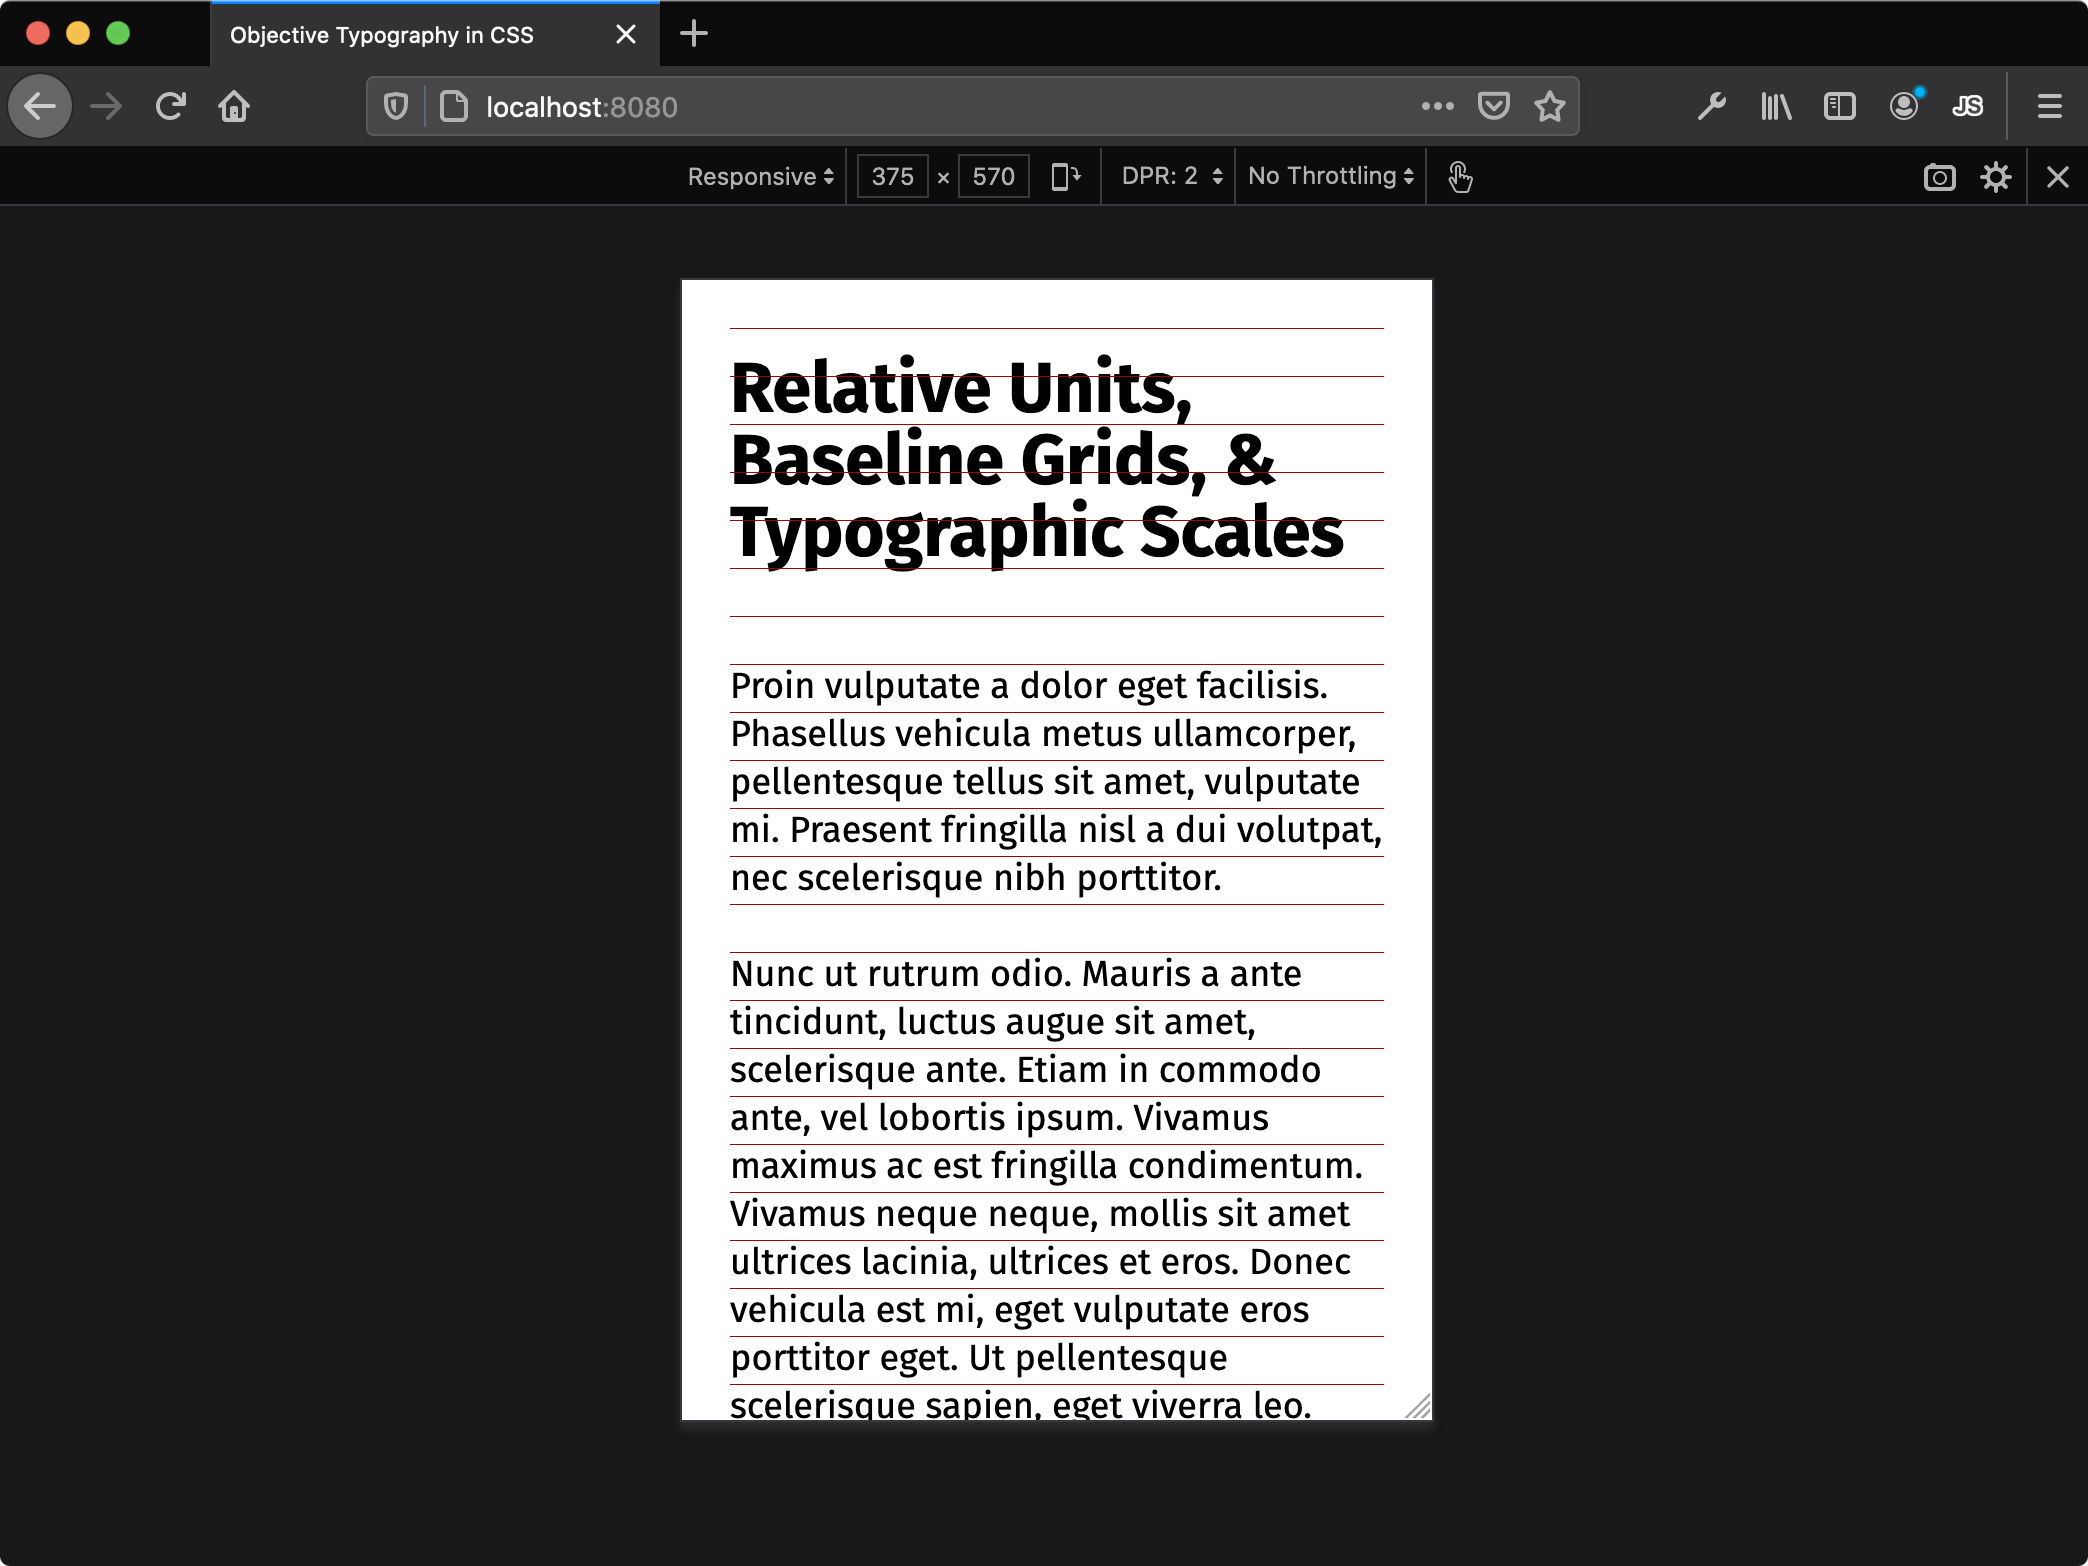
\includegraphics[width=\linewidth]{rdv-narrow}
  \caption{Text precisely set on a repeating baseline grid, with diagnostic grid lines shown. The larger heading text occupies multiple grid lines, while each line of paragraph copy occupies just a single line.}
  \label{fig:rdv-narrow}
\end{figure}

Students begin by working with the responsive design view (RDV) in a development browser such as Mozilla Firefox Developer Edition (Figure \ref{fig:rdv}). The RDV provides an exact readout of the viewport's current size, and protects students from the common pitfall of designing for the web only at the maximum browser-viewport size their computers can display. The viewport in the RDV should be collapsed to a size that approximates the dimensions of a mobile phone. Students need to be reminded of this often.

As an emulator, the RDV has its limitations, so it is important that students also regularly view their work in progress on actual mobile and tablet devices. I require students to make use of a lightweight local web server, such as the \verb|http-server| package written for Node.js \cite{npm:http}, so that they can learn as early as possible to view projects in progress over the local network on other devices, not just in their own chosen development browser. It is usually only when students look at their work on a phone that they begin to really grasp designing for the smallest screens first. The HTML students create or work with should use the viewport \verb|<meta>| element to set mobile devices to display at their native resolutions \cite{mdn:mvp}.

Later in the process, students open up the RDV to simulate page-display on larger viewports and make targeted adjustments to their stylesheets using CSS media queries, as described below, at the end of Section 3.6. That practice better ensures an optimal text setting across a wide range of device and viewport sizes.

\subsection{Sizing Body Type}

Selecting a readable size for body type is a critical step in the typesetting process, because that size value determines all of the other values that follow. Students are typically surprised to learn that there isn’t a precise, universally readable size value. That is due in part to how typefaces are drawn: the optical size of a typeface (that is, its visible letterforms) differs from its body size (the invisible boxes around letterforms, which is what the \verb|font-size| property sets). That means that two typefaces set to the same exact \verb|font-size| value may nevertheless render at different optical sizes. For that reason, in lab assignments I will often require a specific typeface for students to use. Students are responsible for choosing their own typefaces for major projects.

Regardless of the typeface to be sized, students are generally more confident and successful in this work when introduced to some additional constraints for sizing text, including common browser defaults and accessibility guidelines. By default, most desktop browsers set their base font size to 16 pixels, which the latest version of the Web Content Accessibility Guidelines (WCAG) identifies as “a reasonable size to assume” \cite{w3c:wcag}. On the larger end of a starting range of sizes, the Lighthouse Guild, formerly the National Association for the Visually Handicapped, recommends a size range of 16 to 18 points, while also noting the optical-size differences between typefaces \cite{lhg:mtl}. At approximately 1.333 CSS pixels per point, an accessible range of values for the base font size runs between 16 and 24 pixels.

Students seem to find it helpful throughout the process to be reminded that pixel values are only temporary convenience values for use at the design stage, when sizing is still in flux. Eventually, as detailed in Section 3.6 below, all pixel units will be converted to relative \verb|em| or \verb|rem| units, and therefore made responsive to users who set their browser's base font size to something other than the 16-pixel default.

\subsection{Establishing the Baseline Grid}

This is often the step where students encounter the most conceptual difficulty. Their experiences setting line-spacing in word processors, for example, have trained students to think in terms of single- and double-spacing. The concept of setting a value on the CSS \verb|line-height| property to establish a baseline grid is very different, and requires repeated classroom demonstrations in addition to specific feedback about the line-height value students choose on labs and projects.

Guiding principles again help students arrive at a reasonable value to set for the line height. Typographic convention sets the base line-height for body text somewhere between 120\% and 180\% of the base font size  \cite[p.~92]{jsm:owt}. The ideal baseline grid accommodates both the size of the body text and the number of words per line, a value known as the {\itshape measure}. A readable measure on a single column of text is often between 45 and 75 characters, including spaces \cite[pp. 26–27]{rb:style}. Lines with smaller measures can be set closer together than those with larger measures, so long as the baseline is doing its primary job: aiding the eye's movement comfortably from the end of one line of text to the beginning of the next.

To visualize those principles, students benefit greatly from the aid of a diagnostic grid-overlay such as can be displayed by Basehold.it or a simple piece of instructor-provided CSS and SVG \cite{basehold}. With lines showing the size of their chosen baseline grid, students can visually confirm its effectiveness and how their type sits within it.

I encourage students to choose values for the \verb|line-height| property that divide evenly into 2 and 4 for expressing half- and quarter-line adjustments between elements, as is described below in Section 3.5. I also encourage students to regularly switch their grid overlay on and off when determining a line height, because the presence of diagnostic lines can make it more difficult for students to assess when they have discovered a value that is most comfortable for reading.

\subsection{Sizing Accent Type}

Up until this point, students have only been setting properties on the \verb|html| selector. With a base font size and a line-height value in hand, students are ready to make size adjustments to structural text features, such as headings.

Without being offered guidance, student would again choose arbitrarily larger sizes on the heading selectors in their stylesheets. A better, rule-governed approach is to encourage students to experiment with different ratios to determine a typographic scale, also known as a modular scale, for mathematically incremented font sizes. Students report enjoying exploring modularscale.com and its simple controls for specifying a base font size and a number of different pre-defined ratios for resizing text \cite{modscale}.

A 1.333 (4:3) ratio, for example, with a base font size of 18px would produce a typographic scale that includes the sizes 13.503px, 18px, 23.994px, 31.984px, and so on, as shown in Figure \ref{fig:modscale}. Advanced students in particular can be puzzled by partial pixels, like 31.984, as only whole pixels can be lit. But that serves as a good instructional reminder that pixel values are convenience values, which will later be converted to relative units. The browser will handle rounding  either unit to whole-pixel values for display.

To keep the baseline grid consistently sized to accommodate varied text sizes, students need to adjust the \verb|line-height| property on text that is larger or substantially smaller than their base font size, as shown in Figure \ref{fig:rdv-narrow}. Assuming a base font size of 18px and a baseline of 22px, a heading set to 23.994px could be set for comfortable reading on a baseline and a half (33px) or on a fully doubled baseline (44px). As Figure \ref{fig:rdv-narrow} shows, the paragraph text continues to adhere to the grid, indicating that the gridline adjustment on the heading was correctly set.

\begin{figure}
  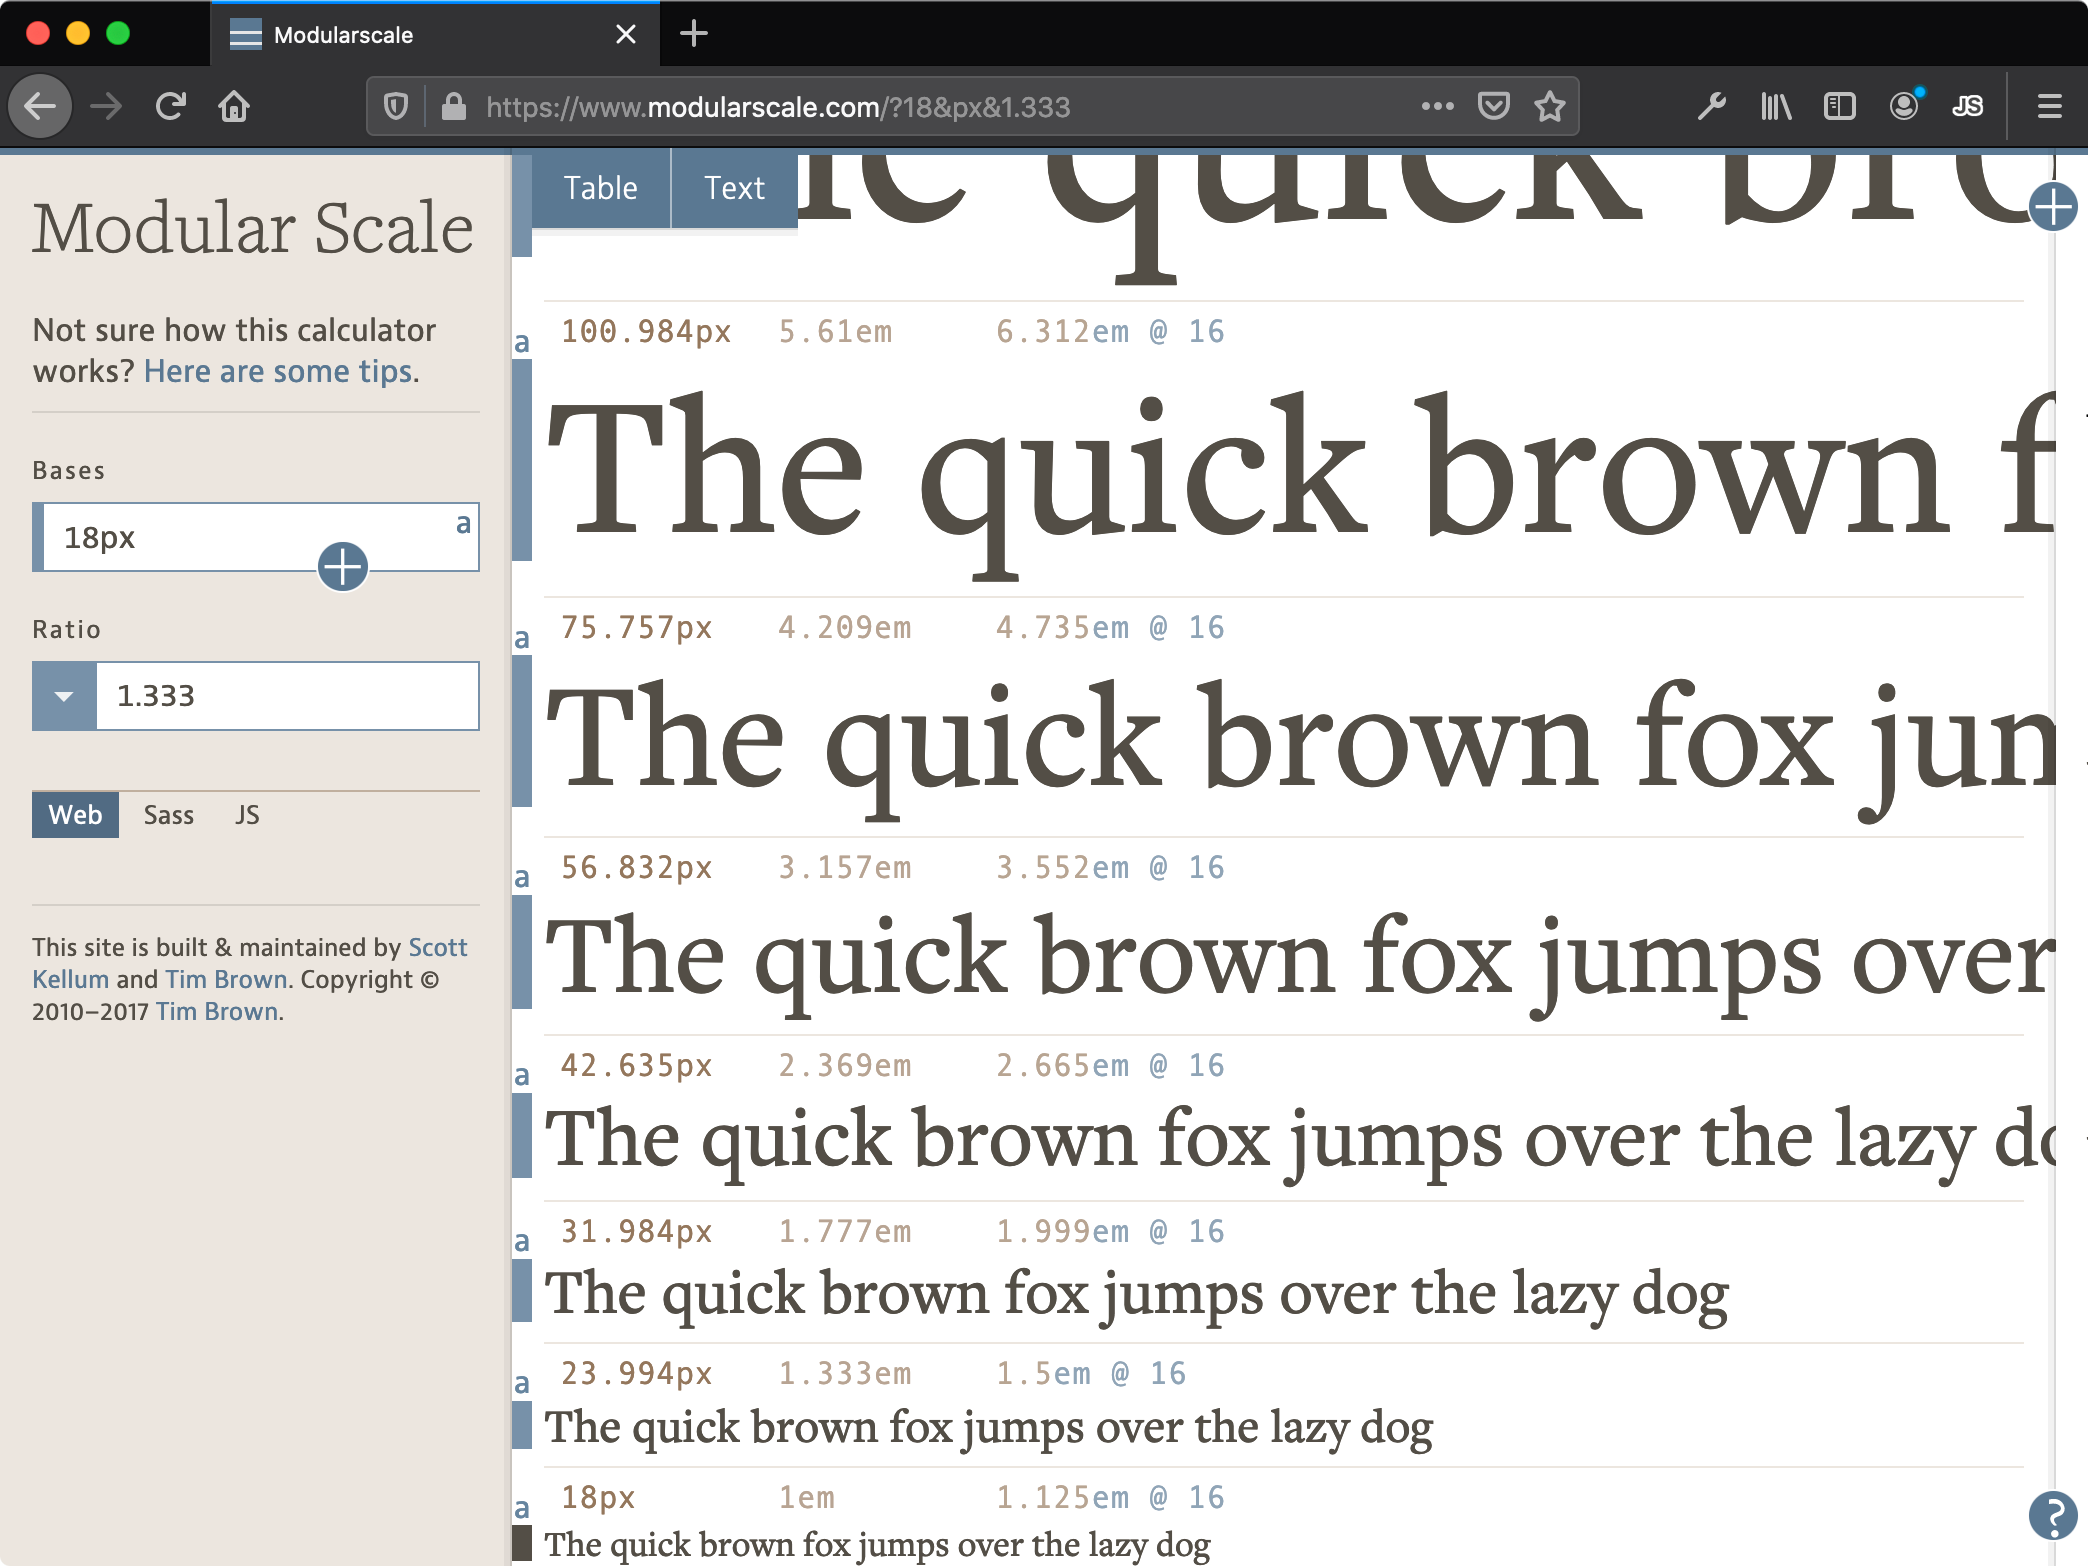
\includegraphics[width=\linewidth]{modular-scale}
  \caption{A 4:3 modular scale with an 18-pixel base font size as shown on modularscale.com.}
  \label{fig:modscale}
\end{figure}


\subsection{Refining the Grid}

Having established a base font size, a baseline grid, and a typographic scale, students move on to adding baseline-determined space around unique structural text elements. Both the \verb|margin| and \verb|padding| properties in CSS are appropriate for this task. I have found that \verb|padding| is better suited to beginners, because it behaves more predictably than \verb|margin|, as CSS collapses adjacent margins under certain conditions.

An entire line of empty space can follow paragraph elements, as shown in Figure \ref{fig:rdv-wide}, while list items can be separated by a half line of space. An additional half line of space set on the list itself ensures that a list, like the paragraphs, will be followed by an entire line of empty space.

\subsection{Relative Units and Responsiveness}

\begin{figure}
  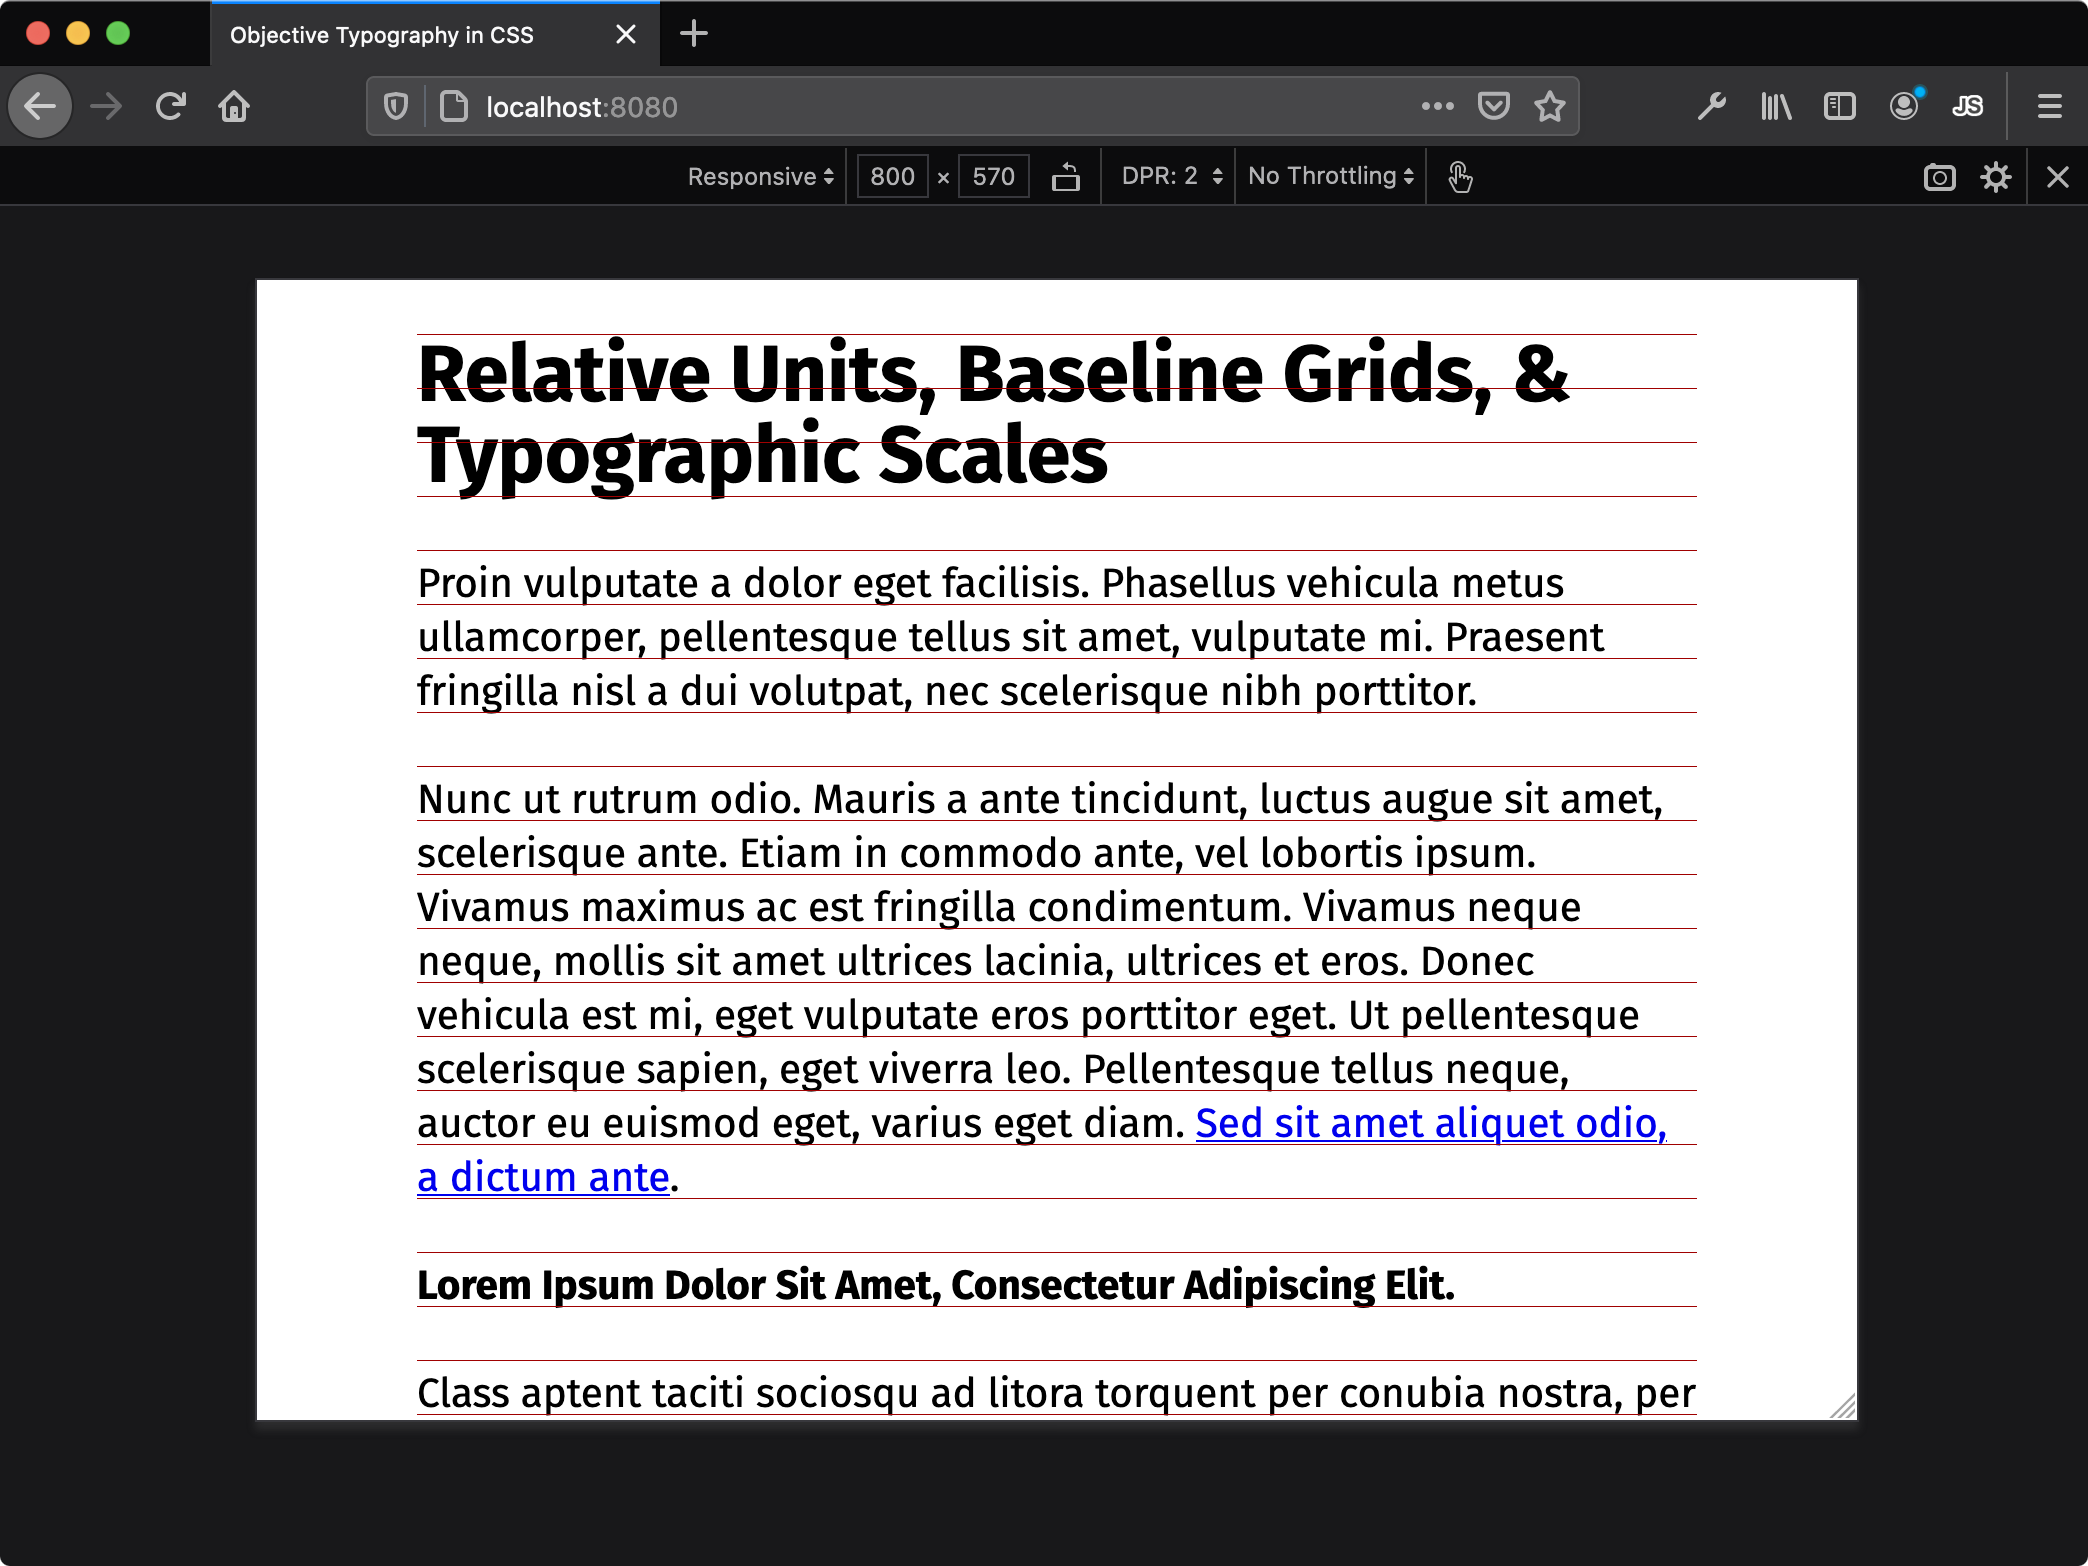
\includegraphics[width=\linewidth]{rdv-wide}
  \caption{Text set larger in a wider RDV viewport, with diagnostic grid lines shown.}
  \Description{At a larger viewport, the text is run larger. Gridlines are still constant, and size relationships between headings and boy copy remain. Additional space appears on either side of the single column of text.}
  \label{fig:rdv-wide}
\end{figure}

With a diagnostic grid overlay still displaying, students begin to gradually convert the values expressed as absolute pixel units to relative em or root em (rem) units. Because browsers default to a 16-pixel em, students convert their base \verb|font-size| value from pixels to ems by dividing by 16. So a 19-pixel \verb|font-size| is equivalent to \verb|1.1875em|.

That value becomes the new em value for the page. If the em-equivalent of 19-pixel text (1.1875em) is set on a 24-pixel baseline, the relative \verb|line-height| value is arrived at by calculating 24 ÷ 19 (not 24 ÷ 16), producing a value of \verb|1.2631578947em|. Students find the shifting value of an em to be confusing, because it changes with each new \verb|font-size| declaration in a stylesheet. The rem unit greatly simplifies calculations for relatively sized text, because it always refers only to the value set on the \verb|html| selector. Unfortunately, the rem unit's support in older browsers is lacking \cite{ciu:rem}. The em unit remains the more widely accessible choice.

With each relative-unit conversion, students should refresh their browsers and ensure their work still shows perfect alignment within the  grid overlay. Any deviations from the grid mean that a relative value was calculated incorrectly.

This is another pain-point for some students, who understandably find the constant browser refreshes tedious--especially because when unit conversions are done correctly, students will see no difference on a refresh. Those students can be tempted to race through their stylesheets and convert everything to relative values without checking their work in the browser. In that situation, students who later discover a problem must return to their stylesheets and check all unit conversions to isolate the source of the errors. I encourage students always to preserve their unit-conversions in CSS comments, which help them to track down errors and to clarify how their relative values were calculated.

With relative units in place, students can then begin to open up the RDV viewport further. Once their lines of text become too long to comfortably read, or exceed the recommended lengths for line measures referenced earlier, an adjustment is needed. CSS media queries are the primary mechanisms for introducing adjustments targeted at specific viewport sizes. Media queries contain CSS that is only applied under a certain screen conditions, such as a minimum width (\verb|min-width|). Students should refer to the width as displayed in the RDV to write the query. A media query may need only to introduce a larger \verb|font-size| set on the \verb|html| selector. All of the carefully determined ratios and size relationships expressed as ems will scale up accordingly. Adding space to the sides of the text column can also help keep the measure of the lines readable, as shown in Figure \ref{fig:rdv-wide}.

\section{Conclusion}

Anecdotally, this approach to CSS instruction has shown itself to be challenging but rewarding for students. Instead of gaining passing knowledge of a growing number CSS of properties, students learn to focus on a set of precise values for a select number of properties. The unique combination of typeface, font size, and line height makes cut-and-paste approaches to CSS unworkable. Students take ownership over their work, and not uncommonly express a great deal of pride when their work scales up with user-set font preferences in the browser. Students also seem more comfortable building on their typesetting knowledge and applying it to grid-based page layout.

In order to formally study the effectiveness of the technique, especially  how it affects student performance with more advanced CSS later in the course, an instrument will be developed and tested in fall 2021 with volunteer students.

\bibliographystyle{ACM-Reference-Format}
\bibliography{stolley.bib}

\end{document}
